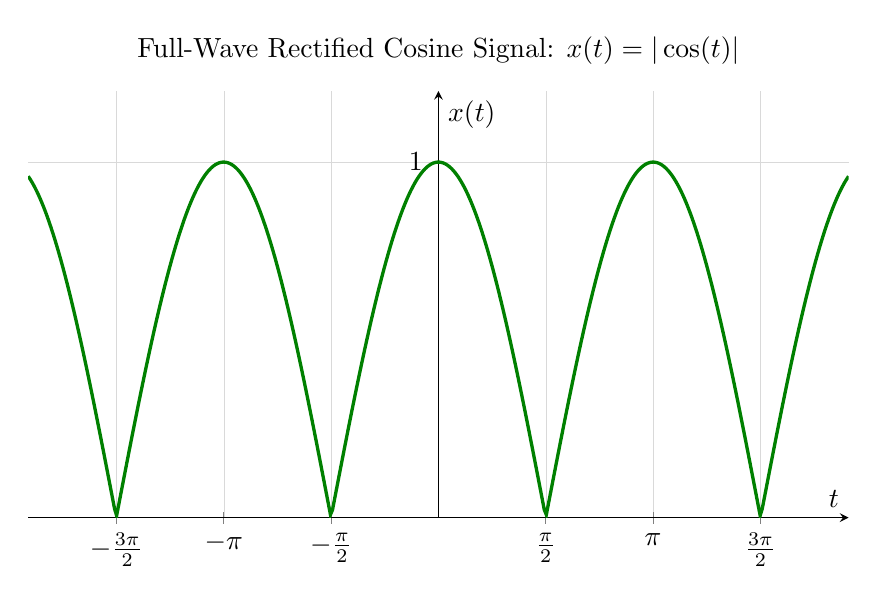
\begin{tikzpicture}
	\begin{axis}[
		width=12cm,
		height=7cm,
		axis lines=middle,
		xlabel={$t$},
		ylabel={$x(t)$},
		title={Full-Wave Rectified Cosine Signal: $x(t) = |\cos(t)|$},
		xmin=-6, xmax=6,
		ymin=0, ymax=1.2,
		xtick={-4.71, -3.14, -1.57, 0, 1.57, 3.14, 4.71},
		xticklabels={$-\frac{3\pi}{2}$, $-\pi$, $-\frac{\pi}{2}$, $0$, $\frac{\pi}{2}$, $\pi$, $\frac{3\pi}{2}$},
		ytick={1},
		yticklabels={$1$},
		grid=major,
		grid style={line width=.1pt, draw=gray!30},
		no marks,
		]
		
		% Plot the absolute value of cosine - multiple periods
		\addplot[green!50!black, very thick, domain=-6:6, samples=400] {abs(cos(deg(x)))};
		
		% Add period labels
		\draw[<->, thick] (axis cs:-3.14, -0.15) -- (axis cs:-1.57, -0.15) node[midway, below=2pt] {$T_0$};
		\draw[<->, thick] (axis cs:-1.57, -0.15) -- (axis cs:0, -0.15) node[midway, below=2pt] {$T_0$};
		\draw[<->, thick] (axis cs:0, -0.15) -- (axis cs:1.57, -0.15) node[midway, below=2pt] {$T_0$};
		\draw[<->, thick] (axis cs:1.57, -0.15) -- (axis cs:3.14, -0.15) node[midway, below=2pt] {$T_0$};
		
	\end{axis}
\end{tikzpicture}